\documentclass[12pt]{report}
\usepackage{graphicx}
\newtheorem{nota}{Nota}

\title{Network+}
\author{Emilio Junoy}
\date{\today}

\begin{document}

\chapter{Modelos de red}
Las redes permiter que los hosts conectados -computadoras- compartan 
recursos y accedan recursos. El sharing host -un servidor- corre
un software espacial que permite al accesing host -un cliente- obtener
el recurso deseado. Ese recurso puede ser varias cosas, desde 
una página Web en el internet hasta archivos en los servidores 
de tu oficina. Inclusive puede ser una impresora o una cámara.\\

Los profesionales de redes usan modelos para conceptualizar las muchas partes
de una red, apoyándose principalmente del modelo Open Systems Interconnection (OSI)
de siete capas.\\

El modelo OSI da dos herramientas que son fundamentales. Primero,
el modelo OSI da una poderosa herramienta mental para diagnosticar problemas.
Entender el modelo OSI permite identificar en qué capa ocurre un error y
permite acercanos a una solución sin muchas vueltas.
Segundo, el modelo OSI da un lenguaje común para que la genete que se 
dedica a las redes pueda hablar sobre funciones específicas de la red.

\section{El modelo OSI en una red sencilla}
Cada capa en el modelo OSI de siete capas define una función importante de 
las redes de computadoras, y los protocolos que operan en esa capa dan soluciones
a esa función. Los $\bf{protocolos}$ son conjuntos de reglas, regulaciones, 
estándares y procedimientos bien definidos que permiten que los 
desarrolladores de hardware y software hagan dispositivos y aplicaciones 
que funciones correctamente en una capa particular. 
El modelo OSI propicia el diseño modular en las redes, lo que significa que cada
capa tiene que hacer la menor cantidad posible de operaciones en las demás capas.
Las siete capas del modelo OSI son:
\begin{itemize}
  \item $\textbf{Capa 7}$ Aplicación
  \item $\textbf{Capa 6}$ Presentación
  \item $\textbf{Capa 5}$ Sesión 
  \item $\textbf{Capa 4}$ Transporte
  \item $\textbf{Capa 3}$ Red 
  \item $\textbf{Capa 2}$ Enlace de datos
  \item $\textbf{Capa 1}$ Fisica
\end{itemize}
Las capas del modelo OSI no son leyes de la física, cualquiera puede diseñar una
red de otra manera. Aunque muchos protocolos encajan exactamente en una capa, 
no todos lo hacen.\\

La mejor manera de entender las capas del modelo OSI es verlas en acción. 
Vamos a verlas en acción con una compañía ficticia llamada MHTechEd Inc.\\

\subsection{¡Bienvenido a MHTechED!}
MHTechED tiene una pequeña red de PCs corriendo Windows, una situación
típica de muchos negocios de hoy en día. Windows viene con todo el software de
redes necesarios para conectarse a una red. Todas las computadoras de MHTechED
están conectadas por un cable especial de red.\\
Como en la mayoría de oficinas, todos en MHTechED tienen su propia PC.
Por el tipo de trabajo que hacen, Shannon y Scott (los administradores)
tienen que mandarse datos entre sus computadoras. En este momento,
Shannon acava de completar un handbook en Word para los empleados y quiere
que Scott lo cheque para ver que sea preciso. Veamos en detalle cada paso 
del proceso que permite que Scott tenga un acceso directo a la computadora 
de Shannon, para que copie el documento de Word del sistema de Shannon al suyo.
Mucho antes de que Shannon siquiera salvara el documento de Word en su sistema
alguien que sabía lo que estaba haciendo configuró todos los sistemas de 
MHTechED para que sean parte de una red común. Toda esta configuración
resultó en múltiples capas de hardware y software que pueden trabajar juntas 
detrás de escenas para que el documento de Word del sistema de Shannon
llegue al sistema de Scott. Examinemos las distintas partes de la red.

\section{Hardware de la red y capas 1-2}
Claramente la red necesita de un canal físico a través del cual se puedan 
mover bits de datos entre los sistemas. La mayoría de redes usan un cable
llamado unshielded twisted pair (UTP), que usualmente contiene cuatro pares 
de cables que pueden transmitir y recibir datos.\\
Otra pieza clave que utiliza la red es un dispositivo en forma de caja que 
maneja el flujo de los datos desde cada computadora hacia cualquier otra.
Esta caja suele estar encerrada en un closet o un cuarto de equipo.
La tecnología de la "central box" ha cambiado con el tiempo. Cada sistema 
tiene un cable que llega a la caja central.\\
La capa 1 del modelo OSI define el método para mover datos entre computadoras,
así que los cables y la "central box" son parte de la $\textit{capa física}$
(capa 1). Cualquier cosa que mueve datos de un sistema a otro, como
cables de cobre, fibra óptica u ondas de radio es parte de la capa física del
modelo OSI. La capa 1 no se preocupa sobre qué datos pasan por ella; solo mueve 
datos de un sistema a otro.\\
La verdadera magia de las redes empieza con la $\textit{network interface card}$
(NIC), que sirve como la interfaz entre la PC y la red. Las hay de distintas formas
y tamaños. En los sistemas más viejos, la NIC era en verdad una tarjeta 
que se conectaba a un slot de expansión en la tarjeta madre.
Los cables y las cajas centrales definen la capa física de la red, y las 
NIC dan una interfaz para la PC.
Podríamos estar tentados a categorizar las NIC como parte de la capa física. 
La NIC es claramente necesaria para que ocurra la conexión física. Muchos autores 
las ponen en la capa 2, así que hay algo interesante pasando con ellas.
\subsection{La NIC}
Para entender las redes, necesitamos entender cómo funcionan las NIC. 
La red debe proveer un mecanismo que le da a cada sistema un identificador 
único -como un número telefónico- para que los datos puedan llega al 
sistema correcto. Ese es uno de los trabajos más importantes de la NIC.
Adentro de cada NIC, quemado dentro de algún chip ROM (Read Only Memory),
hay un firmware especial que contiene un identificador único de 48-bits (6 bytes)
que es llamado la dirección Media Access Control (MAC) de la NIC.\\
No hay dos NICs con la misma dirección MAC, nunca. Cualquier compañía que 
hace NICs debe contactar al Institute of Electrical and Electronic Engineers
(IEEE) y pedir un bloque de direcciones MAC, que la compañía luego quema
en los ROMs de sus NICs. Muchos creadores de NICs también imprimen la 
dirección MAC en la superficie de sus NICs. Notemos que las NICs muestran 
la dirección MAC en notación hexadecimal. Cada dígito de un número hexadecimal 
puede almacenar hasta 16 números, es decir, usa 4 bits de espacio y, como
la dirección MAC es un número de 48-bits, entonces utiliza 12 dígitos hexadecimales.
Las direcciones MAC son del estilo "9c:fc:e8:f3:8a:27". Los primeros seis dígitos, 
en este ejemplo "9c:fc:e8" representan el número del manufactor del NIC. 
Una vez que el IEEE asigna esos seis dígitos a un manufactor -referidos como 
el Organizationally Unique Identifier (OUI)- ningún otro manufactor los puede usar.
Los últimos seis dígitos son el número de serie de esa NIC; a esta parte de la MAC
le llamamos el Device ID.\\
Si tenemos un sistema Windows, podemos usar el comando $\textbf{ipconfig /all}$
desde la terminal para mostrar la dirección MAC. Nota que ipconfig le llama 
dirección física a la dirección MAC, lo cual es una distinción importante.
Para mac (o linux) podemos usar el comando $\textbf{ifconfig}$ y para linux podemos
usar este mismo (si tenemos netutils instalado) o $\textbf{ip a}$.

\subsection{MAC-48 y EUI-48}
El Institue of Electrial and Electronic Engineers (IEEE) forma las direcciones 
MAC de un numbering name space originalmente llamado MAC-48, que simplemente 
significa que la mac es de 48 bits, con los primeros 24 bits definiendo 
el Organizationally Unique Identifier (OUI), como se describió.
El término actual para este numbering name space es EUI-48. 
EUI significa Extended Unique Identifier.
La mayoría de personas les llaman simplemente deirecciones MAC.
Entonces, cada NIC en el mundo tiene una única dirección MAC, pero ¿cómo se utiliza?
Aquí es donde comienza la diversión. Recordemos que los datos de computadoras
son binarios, lo que significa que están hechos de líneas de ceros y unos.
Los NICs mandan y reciben estos datos binarios como pulsos de electricidad, luz u
ondas de radio. Consideremos los NICs que usan electricidad para mandar y recibir
los datos. El proceso exacto mediante el cual un NIC utiliza electricidad
para mandar y recibir datos es excesivamente complicado. En su lugar, 
pensemos una carga en un cable como un 1 y la ausencia de una carga como un 0.
Una vez que entendemos cómo se mueven los datos a lo largo del cable, la siguiente
pregunta es, ¿cómo la red manda los datos correctos al sistema correcto?
Todas las redes mandan los datos rompiendo lo que sea que se esté moviendo
a través de la capa física en cachos discretos llamados $\textit{frames}$.
Un $\textit{frame}$ es básicamente un contenedor para un pedazo de datos que se 
mueven por una red. Un frame $\textit{encapsula}$ la información y los datos
para que tenga una transmisión más sencilla. La NIC crea y manda, así como
recibe y lee estos frames.\\
Aquí es cuando las direcciones MAC se vuelven importantes. A continuación vemos 
una representación de un frame genérico, una versión simplificada 
de la tecnología de red cableada llamada ethernet.
\begin{figure}[h]
  \centering
  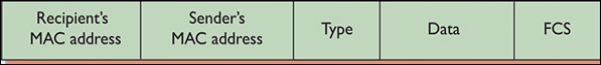
\includegraphics[width=0.8\textwidth]{Frame.png}
  \caption{Frame genérico}
  \label{fig:image}
\end{figure}
Aunque un frame es una string de ceros y unos, frecuentemente dibujamos a los
frames como una serie de rectángulos, cada rectánuglo representando una parte
del string de ceros y unos.\\
Notemos que el frame comienza con la dirección MAC de la NIC a la cual se 
le enviaron los datos, seguido de la dirección MAC del emisor. Despuès 
viene un campo $\textit{Type field}$, que indica lo que está encapsulado 
en el frame. Después biene el campo de $\textit{Data}$ que contiene los datos
que están siendo encapsulados, seguido de un cacho especial de chequeo de información
llamado el $\textit{frame check sequence}$ (FCS). EL FCS usa un tipo de 
matemática binaria llamada $\textit{cyclic redundancy check}$ (CRC) que el NIC
receptor usa para verificar que los datos llegaron intactos.\\
Podemos pensar un frame como teniendo tres secciones. El header, 
que contiene la dirección MAC del receptor, la dirección MAC del emisor y el 
campo data type, en ese orden; el payload, que es lo que está siendo encapsulado 
por el frame y el triales, que es el frame check sequence (FCS).\\
Así que, ¿qué esta dentro de la parte data en el frame? El NIC ni sabe ni le importa.
Los datos podrían ser parte de un archivo, un cacho de un sitio web o un
trabajo de impresión. A los NICs no les importa el contenido. El NIC
simplemente toma los datos que le pasan mediante su device driver y lo manda 
al sistema correcto. Software especial se encarga de qué datos en envían y
qué pasa con los datos cuando llegan.\\
Como una caja, un frame sólo puede guardar una cierta cantidad de datos. 
Distintos tipos de redes usan distintos tamaños de frames, pero los frames utilizados
en redes Ethernet guarda, a lo más, 1500 bytes de información.
Esto genera una nueva pregunta, ¿qué pasa si queremos enviar más datos
que lo que permite el tamaño del frame? Bueno, el software del sistema emisor
debe romper los datos en cachos del tamaño de un frame, que luego pasa al NIC
para su emisión. Conforme el receptor empieza a aceptar información, el software
del receptor recombina los cachos de datos conforme llegan de la red.
\subsection{A la caja central}
Cuando un sistema manda un frame hacia la red, el frame llega a la caja central.
Lo que pasa después depende de la tecnología de la caja central.\\
En el principio de las redes, la caja central era llamada un $\textit{hub}$. 
Un hub era un dispositivo tonto, esencialemente un repetidor. Cuando recibía
un frame, el hub hacía una copia exacta de ese frame y mandaba una copia del
frame original a través de todos los puertos conectados salvo el puerto en el que
se originó el mensaje.\\
La parte interesante del proceso era cuando la copia del frame llegaba a todos
los sistemas. Sólo la NIC a la cual iba dirigido el mensaje procesaba ese frame,
las otras NICs simplemente lo tiraban cuando veían que no estaba dirigido 
a su dirección MAC. Esto es importante de apreciar: con un hub, cada frame mandado 
por la red era recibido por cada NIC, pero sólo la NIC con la dirección MAC 
correspondiente procesaba ese frame.\\
Las redes posteriores reemplazaron los hubs con un dispositivo más inteligente 
llamado switch. Los switches, como veremos más adelante, filtran el tráfico por dirección MAC.
En lugar de mandar todos los frames a todas las NICs conectadas, un switch 
manda el frame sólo a la NIC con la MAC correspondienteprocesaba ese frame,
las otras NICs simplemente lo tiraban cuando veían que no estaba dirigido 
a su dirección MAC. Esto es importante de apreciar: con un hub, cada frame mandado 
por la red era recibido por cada NIC, pero sólo la NIC con la dirección MAC 
correspondiente procesaba ese frame.\\
Las redes posteriores reemplazaron los hubs con un dispositivo más inteligente 
llamado switch. Los switches, como veremos más adelante, filtran el tráfico por dirección MAC.
En lugar de mandar todos los frames a todas las NICs conectadas, un switch 
manda el frame sólo a la NIC con la MAC correspondiente.

\subsection{FCS a profundidad}
Todos los Frame Check Sequence (FCS) tienen sólo 4 bytes, sin embargo
los frames tienen, a lo más, 1500 bytes de datos. ¿Cómo pueden 
4 bytes decir si los 1500 bytes en los datos son correctos? 
Aquí entra la magia matemática del Cyclic Redundancy Check (CRC).
Sin entrar en detalles, podemos pensar en el CRC como un problema de
residuo tras la división. El NIC que manda el frame hace la matemática 
para crear el CRC. El NIC receptor aplica la misma matemática,
si el resultado es igual al CRC, sabe que los datos llegaron bien, de lo contrario,
tira el frame.

\subsection{Llevando los datos a la línea}
El proceso de llevar los datos al cable y luego agarrar esos datos del mismo
es increiblemente complejo. Por ejemplo, ¿qué pasa para que dos NICs no 
hablen al mismo tiempo? Como todos los datos mandados por una NIC son leídas
por todas las demás de la red, sólo un sistema puede hablar a la vez en las redes cableadas 
viejas. Las redes usan frames para restringir la cantidad de datos que una NIC
puede mandar a la vez, dándole a todos los NICs un espacio para que manden 
sus frames por la red en un tiempo razonable.
Tratar con estos y otros problemas requiere de electrónicos sofisticados, 
pero las NICs manejan estos problemas por su propia cuenta.

\subsection{Empezando a conocerte}
Usar las direcciones MAC es una gran manera de mover los dato, pero esto
genera una pregunta importante. ¿Cómo puede una NIC emisora saber cual es la direccion MAC 
de la NIC a la que le está enviando los datos? En la mayoría de los casos,
el sistema emisor ya sabe la dirección MAC pues, probablemente, se habían comunicado antes y
cada sistema guarda estos datos. Si no conoce la dirección MAC, una NIC puede mandar 
un $\textit{broadcast}$ a la red para preguntarlo.
La direccion MAC ff:ff:ff:ff:ff:ff es la dirección de broadcast de la capa 2
-si una NIC manda un frame a la dirección de broadcast, cada NIC en la red procesa ese frame.
Los datos de ese frame de broadcast contiene una petición para la dirección MAC de un sistema.
Sin saber la dirección MAC para empezar, la computadora emisora usará una dirección IP 
para localizar la computadora de entre todas. El sistema con la dirección MAC que está buscando el sistema
leerá la petición en el frame de broadcast y responderá con su dirección MAC.

\subsection{El movimiento de un frame}
Ahora que hemos visto todas las partes que se utilizan para mandar y recibir frames,
pongamos todas las piezas donde van y veamos como llega un frame de un sistema a otro.
El proceso de emisión/recepción básico es como sigue.
Primero, el sistema operativo del sistema emisor pasa algunos datos a su NIC.
La NIC construye un frame para transportar los datos al NIC receptor.
Una vez creado el frame, añade el Frame Check Sequence (FCS) y pone los datos en el frame.
Después, el NIC pone su propia dirección MAC en el frame seguida de la dirección MAC
receptora. Luego manda este frame por los cables de la red.

\begin{nota}
Cualquier frame que va dirigido específicamente a la dirección 
MAC de otro dispositivo es llamado un frame unicast.
\end{nota}
El frame se propaga por el cable de la red hacia la caja central. 
El switch manda frames unicast a la dirección MAC y manda broadcast frames
a cada sistema de la red. La NIC recibe el frame. La NIC le quita la información 
del frame al frame y manda los datos al software - el sistema operativo- para procesarse.
A la NIC receptora no le imprta qué hace el software con los datos, su 
trabajo acaba en el momento en el que pasa los datos al software.\\
Cualquier dispositivo que trabaja con direcciones MAC es parte 
de la capa de enlace de datos del modelo OSI o la capa 2.\\
Notemos que el cableado y los hubs son parte de la capa física. 
Los switches manejan el tráfico usando direcciones MAC, así que operan en ç
la capa 2. Esa es la forma en la que funcionan las redes cableadas modernas.
El NIC está en la capa de enalce de datos y en la capa física.

\subsection{Los dos aspectos de las NIC}
Consideremos como se mueven los datos hacia dentro y hacia afuera de la NIC.
Por un lado, los frames entran y salen de la NIC por su cable de red. 
Por otro lado, los datos se mueven hacia arriba y hacia abajo entre la NIC
y el software de red del sistema operativo. Los muchos paso sque la NIC 
hace para mantener estos datos en movimiento - mandar y recibir datos por el cable,
crear frames salientes, recibir frames y agregarles las direcciones MAC- están 
divididos en dos trabajos distintos.\\
El primer trabajo es llamado Logical Link Control (LLC). 
El LLC es el aspecto de la NIC que habla con el sistema operativo (usalmente mediante drivers
del dispositivo). El LLC maneja múltiples protocolos de red y provee control de flujo.\\
El segundo trabajo es llamado Media Access Control (MAC), que 
crea y dirige los frames. Añade su propia dirección MAC y las direcciones MAC 
a los frames. La subcapa de MAC añade o checa el Frame Check Sequence (FCS).
La MAC también se asegura de que los frames, ahora completos con su dirección MAC,
sean mandados por los cables de la red.

\subsection{NIC y capas}
La mayoría de materiales de redes que describen el modelo OSI ponen
a las NICs en la capa de enlace de datos del modelo. 
Es en la subcapa MAC, después de todo, que los datos son encapsulados en un frame,
las MACs de destino y emisión son agregadas al frame y ocurre el chequeo de errores.
Lo que molesta a muchos estudiantes de poner las NICs únicamente en la capa 
de enlace de datos es la obvia tarea de las NICs de poner ceros y unos en el cable o en el aire.
Pero las NICs operan en ambos niveles.

\section{Más allá del cable -software de red y capas 3-7}
Llevar datos de un sistema a otro en una red simple (una en la que todas las computadoras
están conectadas al mismo switch) toma poco esfuerzo por parte de las NICs.
Pero un problema con las redes simples es que las computadoras deben hacer broadcast
para obtener las direcciones MAC. Funciona para redes pequeñas, pero que pasa si las redes 
son grandes, como del tamaño de todo el internet.\\
De igual manera, los datos fluyen usando muchas tecnologías, no solo Ethernet.
Estas tecnologías no saben que hacer con las direcciones MAC del Ethernet. 
Cuando las redes se vuelven grandes, no podemos usar direcciones MAC.\\
Las redes grandes necesitan un método de logical addressing, como un código postal
o un esquema de números telefónicos, que ignora el hardware y permite 
romper la red completa en cachos más pequeños llamados subredes.\\
Para movernos más allá de las direcciones MAC y empezar a usar
logical addressing, se requiere un software espacial llamado protoclo de red.
Los protocolos de red existen en cada sistema operativo. 
Un protocolo de red no sólo debe crear identificadores únicos para cada sistema,
pero debe también crear un conjunto de reglas de comunicación para problemas como
cómo manejar datos que están rotos en múliples paquetes y cómo asegurarse 
de que los paquetes lleguen de una subred a otra.
Tomemos un momento para aprender un poco sobre la colección más famosa
de protocolos de red -TCP/IP- y su sistema de unique addressing universal.

\begin{nota}
Las direcciones MAC son también llamadas direcciones físicas
\end{nota}

Para ser precisos, TCP/IP es, en realidad, varios protocolos diseñados para trabajar juntos,
mejor conocido como una suite de protocolos, pero dos protocolos, TCP  e IP hacen tanto
trabajo que decidieron llamar a la suite con este nombre.\\
TCP significa $\textit{Transmission Control Protocol}$ e 
IP significa $\textit{Internet Protocol}$. IP es el protocolo de red
que debemos discutir primero.

\subsection{IP-jugando en la capa 3}
En la capa de red, la capa 3, los contenedores llamados paquetes son creados 
y dirigidos para que puedan llegar de una red a otra. El Internet Protocol
es el protocolo de logical addressing principal para TCP/IP.
IP se asegura de que un pedazo de datos llegue a donde tiene que llegar en la red.
Hace esto dándole a cada dispositivo en la red un identificador numérico 
único llamado dirección IP. Una dirección IP es conocida como dirección lógica, 
para distinguirla de las direcciones físicas, las direcciones MAC de las NICs.\\
IP usa una notación decimal basada en cuatro numeros de 8-bits.
Cada número de 8 bits está en el rango de 0 a 255 y los números están separados por puntos.
Un ejemplo de dirección IP es $\textit{192.168.1.76}$.\\
No hay dos sistemas en la misma red que compartan direcciones IP;
si dos máquinas reciben la misma dirección IP por accidente, podrían ocurrir
efectos no deseados. Estas direcciones IP no aparecen mágicamente -deben ser configuradas
por el administrados.\\
Lo que hace poderoso al logical addressing es otra caja mágica, llamada router, que conecta
cada una de las subredes. Los routers usan las direcciones IP, no las direcciones MAC, para
mandar los datos. Esto permite que las redes se conecten a lo largo de líneas de datos que no
usan Ethernet, como las lineas de teléfono. Cada tipo de red (como Ethernet, SONET y otros)
usan un frame único.\\
En una red TCP/IP, cada sistema tiene dos identificadores únicos: la direcciòn MAC y 
la dirección IP. La dirección MAC (la dirección física) literalmente
está quemada en los chips de las NICs, mientras que las IP (la dirección lógica)
está almacenada en el software del sistema. Las direcciones MAC vienen con las NICs, así que 
no hay que configurarlas, pero las direcciones IP sí hay que configurarlas.

\subsection{Paquetes dentro de frames}
Para que una red TCP/IP mande datos de forma exitosa, los datos
deben estar envueltos en dos contenedores distintos.
Un frame de algún tipo permite que los datos se muevan de un 
dispositivo a otro. Dentro de ese frame hay un contenedor IP-específico
que permite que los routers determinen a dónde mandar los datos
-independientemente del tipo de conexión física- y los datos mismos.
En TCP/IP, el contenedor interno es un paquete.

\begin{figure}[h]
\centering
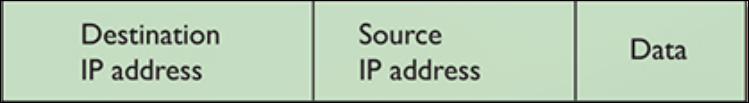
\includegraphics[width=0.8\textwidth]{Paquete.png}
\caption{Paquete IP}
\end{figure}

Pero los paquetes IP no se van desnudos. Cada paquete IP es entregado
a la NIC, que depués lo encapsula dentro de un frame normal,
en esencia, un paquete dentro de un frame.

\begin{figure}[h]
\centering
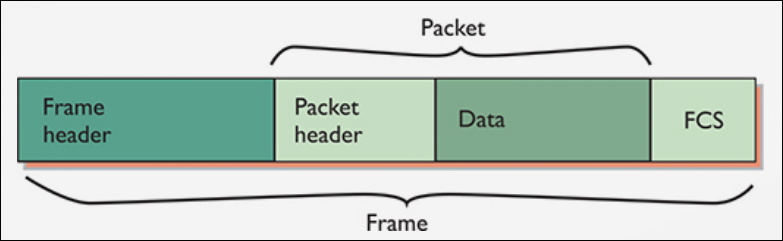
\includegraphics[width=0.8\textwidth]{Frame-Paquete.png}
\caption{Paquete IP dentro de un frame}
\end{figure}

Cuando mandamos datos de una computadora a otra en una red TCP/IP
como el internet, esos datos pueden pasar por muchos routers antes
de llegar a su destino. Cada router quita el frame que le llega, determina
a dónde mandar los datos de acuerdo con la dirección IP del paquete,
crea un nuevo frame y manda ese paquete dentro del frame a la siguiente 
parada. El nuevo tipo de frame será de la tecnología apropiada para
que llegue al siguiente router. Podría ser un cable o una conexión 
DSL. El paquete IP, por otro lado, permanece sin cambiarse.\\
Una vez que el paquete llega al router de la subred de destino, 
ese router quita el frame, ve la IP de destino, y añade un frame
con la dirección MAC apropiada para esa dirección IP.\\
La NIC receptora queita el frame de Ethernet y pasa el paquete al 
software. El software de red del sistema operativo hace el resto.
El software del driver de la NIC es la interconexión entre el hardware
y el software. El driver del NIC sabe como comunicarse con la NIC para 
mandar y recibir frames, pero no puede hacer nada con los paquetes.
En su lugar, el driver del NIC manda el paquete a otros servicios
que saben cómo manejar los paquetes para convertirlos en páginas web,
mensajes de e-mail, archivos y demás.

\subsection{Segmentación y reensamblado -Capa de transporte, capa 4}
Como la mayoría de bloques de datos son mucho más grandes que un 
solo paquete, deben ser rotos antes de que se pueden mandar por la red.
Cuando una computadora "serving" recibe una petición para algunos datos,
debe ser capaz de romper los datos pedidos en bloques que quepan
dentro de un paquete (y eventualmente en un frame de una NIC),
organizar los paquetes para el beneficio del sistema receptor, y darlos
a la NIC para enviar. Esto es llamado $\textit{segmentación}$.
El sistema receptor hace el $\textit{reensamlado}$ de los paquetes.
Debe reconocer una serie de paquetes como una transmisión de los mismos datos,
reensamblar los paquetes correctamente basandose en la información 
incluida en los paquetes del sistema emisor, y verificar que todos
los paquetes de un pedazo de datos lleguen de buena manera.\\
Esta parte es relativamente sencilla -el protocolo de transporte 
rompe los datos en cachos llamados segmentos y le da a cada segmento
un tipo de número de secuencia. (Los datagramas, también creados en la capa 4,
son más simples y no necesitan romperse ni que se les de números
de secuencia).\\
Encajado en los datos de cada paquete hay un número de secuencia.
Leyendo los números de secuencia, el sistema receptor sabe cuántos segmentos
hay y cómo ensamblarlos de forma correcta.\\
La capa 4, la capa de transporte tiene un papel muy importante: 
es el software de segmentación/reensamblado. Parte de su trabajo es pedir
los paquetes que no se recibieron en el orden correcto.

\subsection{Comunicación basada en conexión vs. sin conexión}
Algunos protocolos, como Simple Mail Transfer Protocol (SMTP) usado
para enviar mensaje e-mail, requieren que el cliente de e-mail y el servidor
establezcan una conexión antes de mandar un mensaje.\\
De otro modo, algunos protocolos TCP/IP simplemente mandan los datos 
sin primero esperar a que el sistema receptor esté listo.
Cuando usamos Voice over IP (VoIP), por ejemplo, la llamada se hace
sin verificar que el otro sistema esté ahí.\\

\begin{nota}
El protocolo orientado a la conexión es el Transmission Control Protocol (TCP).
El protocolo sin conexión es el User Datagram Protocol (UDP).
\end{nota}

\subsection{Segmentos dentro de paquetes}
Para ver la capa de transporte en acción, hay que quitar las direcciones IP
del paquete IP. Lo que nos queda es un bloque de datos dentro de otro contenedor,
llamado un $\textit{Segmento TCP}$. Los segmentos TCP tienen muichso otros campos
para asegurarse de que los datos lleguen al destino en el orden correcto.
Estos campos tienen nombres como Puerto de salida, Puerto de destino,
Número de secuencia, Número de Ackwnoladgement.

\begin{figure}[h]
\centering
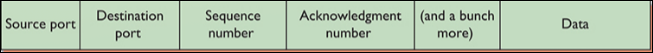
\includegraphics[width=0.8\textwidth]{Segmento.png}
\caption{Segmento TCP}
\end{figure}

En este contexto, un $\textit{puerto}$ es un número entre 1 y 65,536,
es un valor lógico asignado a aplicaciones o servicios específicos.
Un ejemplo dejará esto claro. Muchos segmentos TCP llegan a una computadora.
La computadora necesita una forma de saber qué segmentos TCP van a qué aplicaciones.
Un servidor web, por ejemplo, ve mucho tráfico, pero escucha a los segmentos TCP
con puerto de destino 80 o 443, agarra esos segmentos y los procesa.
De igual manera, todo segmento TCP contiene otro número de puerto, el puerto de salida,
para que el cliente sepa que hacer para regresar la información.\\
Los datos vienen de la capa de aplicación (con algo de input de las capas
de presentación y sesión). La capa de tranporte rompe esos datos en bloques,
añadiendo núemeros de puerto y números de sucesión, creando un segmento TCP.
La capa de tranporte luego manda el segmento TCP a la capa de red, que crea un paquete
IP.\\
Aunque mucho tráfico de una red TCP/IP usa TCP en la capa de tranporte, 
hay otro protocolo, el User Datagram Protocol. Siguiendo el mismo proceso,
la capa de transporte añade números de puertos, un número de longitud y 
un checksum como headers y combina esto con los datos para crear un contenedor
llamado un datagrama UDP. Un datagrama UDP no tiene la mayoría de campos
que utilizan los segmentos TCP, simplemente porque a UDP no le importa 
si la computadora receptora recibe los datos.

\begin{figure}[h]
\centering
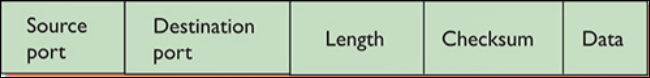
\includegraphics[width=0.8\textwidth]{Datagrama.png}
\caption{Datagrama UDP}
\end{figure}

\subsection{Hablando en la red - Capa 5, la capa de sesión}
En una red, un sólo sistema puede estar hablando con muchos otros al mismo tiempo.
Por ejemplo, la PC de Shannon tiene una impersora usada por todos los sistemas
de MHTechED, así que existe la posibilidad de que cuando Scott intente 
acceder al documento Word, otro sistema está mandando un trabajo de impresión 
a la PC de Shannon.\\
El sistema de Shannon debe dirigir estos archivos, trabajos de impresión,
páginas web y demás a los programas adecuados. Adicionalmente,
el sistema operativo debe permitir que un sistema haga una conexión 
con otro sistema para verificar que el otro sistema pueda manejar lo que sea que 
sistema inicial quiera hacer. Si el sistema de Bill quiere mandar un 
trabajo de impresión a la impresora de Shannon, primero contacta
a la computadora de Shannon para saber si puede manejar el trabajo de impresión.
El software de sesión maneja esta parte de las redes, conectando 
aplicaciones a aplicaciones.\\

\subsection{Ve tus sesiones}
¿Cuántas sesiones tiene un sistema típico corriendo al mismo tiempo?
Bueno, si tienes una red TCP/IP, puedes correr el programa netstat 
desde la línea de comandos para verlos todos. Abre una línea de comandos y escribe
$$\textbf{netstat -a}$$
Después presiona enter para ver las sesiones. Por ahora, simplemente aprecia que cada línea
del output de netstat es una sesión. En linux también podemos correr el comando ss
La capa de sesión, la capa 5 del modelo OSI, maneja todas las sesiones para un sistema.
La capa de sesión inicia las sesiones, acepta sesiones entrantees y abre y cierra las sesiones
existentes.\\
Muchos sistemas operativos representan las sesiones usando una combinación
de las direcciones IP y los números de puertos de ambos lados de la comunicación 
TCP o UDP. Podemoms ver la sesión de un buscador web conectándose a un servidor web,
por ejemplo, corriendo $\textbf{netstat -n}$. Regresará muchas líneas como esta:
$$\textbf{TCP 192.168.4.34:45543     11.12.13.123:80    Established}$$

Los números describen la sesión. Un cliente web con dirección IP 
192.168.4.34 uando el puerto 45543, está en una sesión TCP con un servidor web
usando la dirección IP 11.12.13.123.

\subsection{Traducción - Capa 6, capa de presentación}
La capa de presentación traduce los datos de las capas más bajas 
a un formato que pueda usar la capa de aplicación y vice versa.
esto se manifiesta de muchas maneras y no es muy claro. Esto pasa porque
las redes TCP/IP no se mapean directamente al modelo OSI.\\
Un número de protocolos funionan en más de una capa del modelo OSI y pueden 
incluir la capa 6, de presentación. El protocolo de encripción usado en el 
e-commerce, Transport Layer Security (TLS), por ejemplo, parece que se empieza
en la capa 5 y luego encripta y desencripta en la capa 6.

\subsection{Aplicaciones de red - Capa 7, la capa de aplicación}
La última capa y la más visible de un ared es el software de las apliciones
que la utilizan. Si queremos copiar un archivo de otro sistema en nuestra red,
necesitamos un applet como Network en Windows 10 que permite 
acceder a archivos de manera remota. Si queremos ver páginas web, debemos usar
un buscador como Google Chrome o Mozilla Firefox. Las personas que usan una red
la experimentan mediante las aplicaciones.\\
Las aplicaciones pueden incluir funciones adicionales, como encripción,
autentificación de usuarios y herramientas para controlar la parte visual de los datos.
Pero estas funciones son específicas a las aplicaciones. 
La capa de aplición es la capa 7 del modelo OSI. Mantén en mente que 
la capa de aplicación no se refiere a las aplicaciones mismas. Se 
refire al codigo incluido en todos los sitemas operativos que permiten 
tener aplicaciones concientes de la red. Todos los sistemas operativos tienen
Application Programming Interfaces (APis) que los programadores pueden usar
para hacer sus programas concientes de la red. Una API, en general, le da 
la capacidad a los programadores de extender las capacidades de sus aplicaciones

\subsection{Encapsulación y desencapsulación}
El término encapsulación engloba todo el proceso de preparar los datos
para que vayan a una red. Esto incluye todos los pasos desde la aplicación a las capas 
de Aplicación, Presentación, Transporte, Red y Enlace de Datos.
Cada capa añade más información para que los datos lleguen al receptor correcto
y que el receptor sepa qué hacer con los datos.\\
La computadora receptora hace el proceso en reversa, quitando la información 
extra de los headers conforme los datos suben por las capas. Este proceso inverso
es llamado desencapsulación.\\
La capa de transporte crea un segmento o datagrama y lo pasa a la capa de red. 
Esa capa añade información de IP, encapsulando el segmento o datagrama en un paquete.
La capa de enlace de datos envuelve todo el paquete en un frame para que sea enviado por al red.
La NIC transforma el frame en bits para la transmisión por el medio.
La NIC receptora recibe los bits y los trasforma en el frame,
el sistema quita la información extra del frame para quedarse con un paquete IP.
Luego, quita la información IP del paquete y se queda con un segmento TCP o un 
datagrama UDP. Después, en el caso de un segmento TCP, ensambla los segmentos
recibidos para pasarlos por la capa de presentación para finalmente llegar a la capa de aplicación.

\section{El modelo OSI de siete capas y el trabajo remoto}
Beth trabaja remotamente para una compañía como analista de datos.
Exploremos su flujo de trabajo para ver cómo aplica el modelo OSI de siete capas.\\
Beth se conecta el internet de forma inalámbrica desde su lapotp.
Su compañía, como muchas otras, usa un número de diferentes servicios 
en línea para coordinar su fuerza de trabajo. Estos servicios tienen
nombres como Microsoft 365, Dropbox, Github, entre otros, pero fundamentalemnte
estos servicios se encuentran en la Web, así que Beth pasa mucho tiempo de su día en su 
buscador de preferencia, Firefox.\\
En este escenario, la computadora de Beth no está conectada a un puerto Ethernet.
No hay cables locales, su laptop ni siquiera tiene un puerto Ethernet.\\
Las ondas de radio inalámbricas conectan a la laptop de Beth a un Wireless Access Point (WAP)
que opera en la capa 1. De igual modo lo hacen todos los cables físicos que conectan su 
WAP a su router, Internet Service Provider (ISP) y todos los routers entre su red y la 
red de su compañía.\\
La NIC inalámbrica de Beth ciertamente tiene una dirección MAC y se conecta a su Wireless 
Access Point (WAP) usndo frames; el WAP usa las direcciones MAC para conectarse al switch local.
Todo esto claramente sucede en la capa 2. Beth hace casi todo su trabajo
via Web y, por lo tanto, depende casi enteramente en conexiones e interacciones 
TCP/IP. Por definición, su laptop debe tener una dirección IP o dos (capa 3) y 
debe encapsular y desencapsular segmentos y datagramas en la capa de transporte (capa 4).
Pero el trabajo duro ocurre en la capa 7 con HTTP y  TLS (HTTPS), pues las herramientas Web
se basan en estos protocolos.\\
En pocas palabras, el modelo OSI de 7 capas nos da una manera de conceptualizar 
las redes para determinar dónde es que se da un cierto error. 
El modelo OSI puede aplicarse a una red simple o a una red más avanzada.\\
Si Beth no puede imprimir con su impresora de red, por ejemplo, un modelo
nos puede ayudar a solucionar el problema. Si su NIC muestra actividad, entonces
usando el modelo OSI, podemos descartar las capas uno y dos. Nos movemos
hacia arriba a la capa 3. Si su computadora tiene una dirección IP propia, podemos poner
esa capa a un lado también y podemos checar las siguientes capas de una en una para 
solucionar el problema.
\begin{nota}
  Beth accede a servidores para hacer su trabajo; su laptop es un cliente
  de esos servidores. Así, el escenario anterior describe una red de tipo cliente-servidor típica.
  En algunas circunstancias, Beth podría acceder a recursos distribuidos entre 
  varias computadoras. Así, su computadora podría compartir recursos con otras.
  Este tipo de red alternativa, tipificado por el protocolo de BitTorrent, 
  es llamado peer-to-peer.
\end{nota}

\section{Preguntas}

\begin{enumerate}
  \item ¿A dónde manda los datos un Hub?
    A todos los sitemas conectados al hub.
  \item ¿Qué identifica de manera única a cada NIC?
    Una dirección Media Access Control (MAC).
  \item ¿Qué comando de Windows usamos para encontrar la dirección MAC de un sistema?
    ipconfig /all
  \item Una dirección MAC es conocida como una direccion ...
    Física
  \item Una NIC manda los datos en bloques llamados ...
    Frames
  \item ¿Cómo empieza un frame?
   Con la dirección MAC del sistema receptor.
  \item Un frame termina con 4 bytes especiales llamados el frame check sequence (FCS). ¿Qué hace el FCS?
    Verifica que los datos llegaron correctamente.
  \item ¿Cuál es un ejemplo de una dirección MAC?
    00-50-56-A3-04-0C
  \item ¿Qué capa del modelo OSI controla la segmentación y el reensamblado de los datos?
    La capa de tranporte (Capa 4)
  \item ¿Qué capa del modelo OSI lleva registro de las conexiones del sitema para llevar los datos a la computadora correcta?
    La capa de sesión (Capa 5)
\end{enumerate}
\end{document}
